\section{Технологический раздел}

\subsection{Выбор реляционной СУБД}

Наиболее популярными реляционными СУБД являются:

\begin{itemize}[leftmargin=0.7cm + \labelwidth - \labelsep]
	\item[---] Oracle \cite{oracle};
	\item[---] MySQL \cite{mysql};
	\item[---] Microsoft SQL Server \cite{sqlserver};
	\item[---] PostgreSQL \cite{postgresql}.
\end{itemize}

Сравнение упомянутых СУБД представлено в таблице \ref{tech:cmpsubd}.

\begin{table}[H]
	\caption{Сравнение реляционных СУБД}
	\label{tech:cmpsubd}
	\small
	\begin{tabular}{|c|c|c|c|c|}
		\hline
		 & Oracle & MySQL & Microsoft SQL Server & PostgreSQL \\ \hline
		Простота в использовании & + & + & + & + \\ \hline
		Бесплатная полная версия & - & - & - & + \\ \hline
		Безопасность данных & + & - & + & + \\ \hline
		Поддержка стандарта SQL & + & + & + & + \\ \hline
		Поддержка процедур и триггеров & + & + & + & + \\ \hline
		Кроссплатформенность & + & + & - & + \\ \hline
	\end{tabular}
\end{table}

Как видно из таблицы \ref{tech:cmpsubd}, PostgreSQL удовлетворяет всем перечисленным критериям, следовательно, может быть использована при управлении разрабатываемой базой данных магазина электроники.

\subsection{Выбор средств реализации}

Для реализации приложения доступа к базе данных был выбран язык программирования Python. Это кроссплатформенный язык с поддержкой объектно-ориентированного подхода, подходящий для работы с PostgreSQL. Выбор также обусловлен знанием возможностей языка, что облегчит процесс написания и отладки кода.

В качестве среды разработки была выбрана Visual Studio Code. Это кроссплатформенная среда с обширным перечнем настроек проекта. Достаточный опыт работы в этой среде разработки, удобства написания кода и его автодополнения стали ключевыми при выборе.

Для создания графического интерфейса приложения было решено использовать Qt Designer, который предоставляет большой набор базовых компонентов, необходимых для решения поставленной задачи.

\subsection{Структура системы}

Разрабатываемая система работает следующим образом: от пользователя поступает запрос, приложение его обрабатывает, данные читаются из базы и записываются в базу с использованием коннектора. Пользователь получает ответ на свой запрос через графический интерфейс.

Структура системы отображена на рисунке \ref{tech:architecture}.

\begin{figure}[H]
	\centering{
		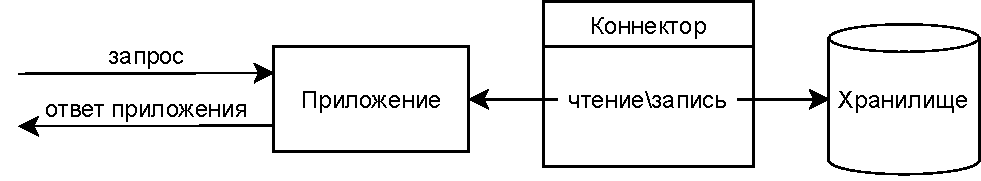
\includegraphics[width=1\textwidth]{img/structure.pdf}
		\caption{Структура системы}
		\label{tech:architecture}}
\end{figure}

\pagebreak

\subsection{Создание базы данных}

В листингах \ref{tech:init1} и \ref{tech:init2} приведен сценарий создания спроектированной базы данных на языке SQL.

\lstinputlisting[
firstline=1,
lastline=26,
caption={Сценарий создания базы данных. Часть 1},
label={tech:init1}
]
{listings/init.sql}

\pagebreak

\lstinputlisting[
firstline=28,
lastline=64,
caption={Сценарий создания базы данных. Часть 2},
label={tech:init2}
]
{listings/init.sql}

\pagebreak

\textbf{Ролевая модель}

Для обеспечения безопасности доступа к данным, на уровне базы создана ролевая модель. Ее реализация показана в листинге \ref{tech:roles}.

\lstinputlisting[
firstline=131,
lastline=155,
caption={Ролевая модель на уровне базы данных},
label={tech:roles}
]
{listings/init.sql}

\pagebreak

\textbf{Триггер для обновления количества товаров}

Реализация триггера для обновления количества товаров отражена в листинге \ref{tech:updateqnt}.

\lstinputlisting[
firstline=75,
lastline=84,
caption={Триггер для обновления количества товаров},
label={tech:updateqnt}
]
{listings/init.sql}

\textbf{Триггер для удаления пользователя системы}

Реализация триггера для удаления пользователя системы отражена в листинге \ref{tech:deluser}.

\lstinputlisting[
firstline=86,
lastline=97,
caption={Триггер для удаления пользователя системы},
label={tech:deluser}
]
{listings/init.sql}

\pagebreak

\subsection{Интерфейс приложения}

Для входа в систему пользователю необходимо ввести логин и пароль. Покупатель не авторизуется в системе, поэтому ему следует оставить поля ввода пустыми. Окно авторизации показано на рисунке \ref{tech:auth}.

\begin{figure}[H]
	\centering{
		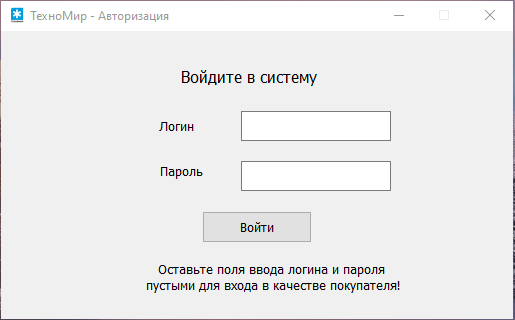
\includegraphics[width=0.45\textwidth]{img/auth.png}
		\caption{Окно авторизации}
		\label{tech:auth}}
\end{figure}

Если войти в систему под учетной записью администратора, то можно получить доступ к списку всех пользователей системы, а также возможность удалять и добавлять их учетные записи, редактировать информацию о пользователях. Интерфейс, доступный администратору, показан на рисунке \ref{tech:admin}.

\begin{figure}[H]
	\centering{
		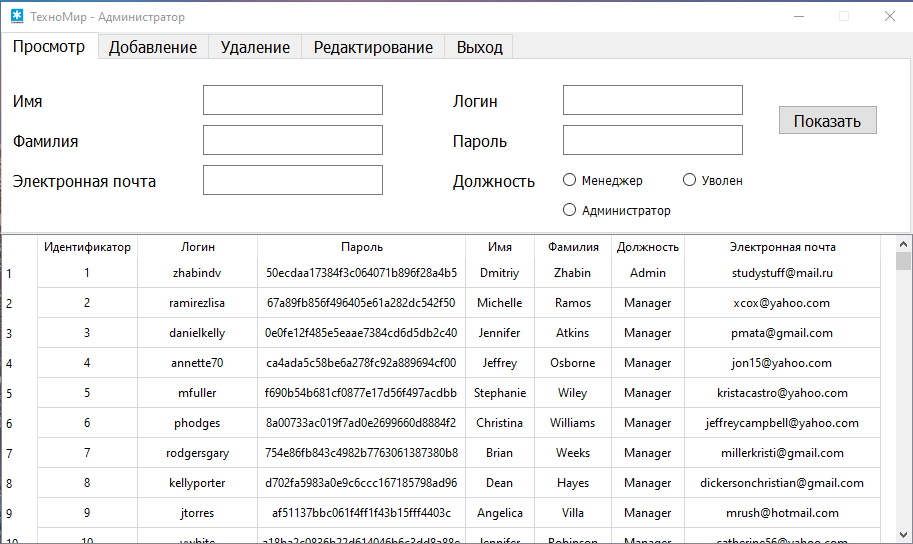
\includegraphics[width=0.95\textwidth]{img/admin.png}
		\caption{Интерфейс администратора}
		\label{tech:admin}}
\end{figure}

Если войти в систему под учетной записью менеджера, то можно получить доступ к каталогу товаров, представленных в магазине. Заполняя поля значений-фильтров, менеджер может найти товары по необходимым параметрам. В этой же вкладке интерфейса менеджер может добавить новый товар в каталог, предварительно заполнив всю информацию о нем, в том числе и сведения о поставщике. Если информация о конкретном поставщике уже есть в системе, то достаточно ввести название организации, оставив поля ввода адреса и номера телефона пустыми. Окно просмотра каталога товаров для менеджера представлено на рисунке \ref{tech:mancat}.

\begin{figure}[H]
	\centering{
		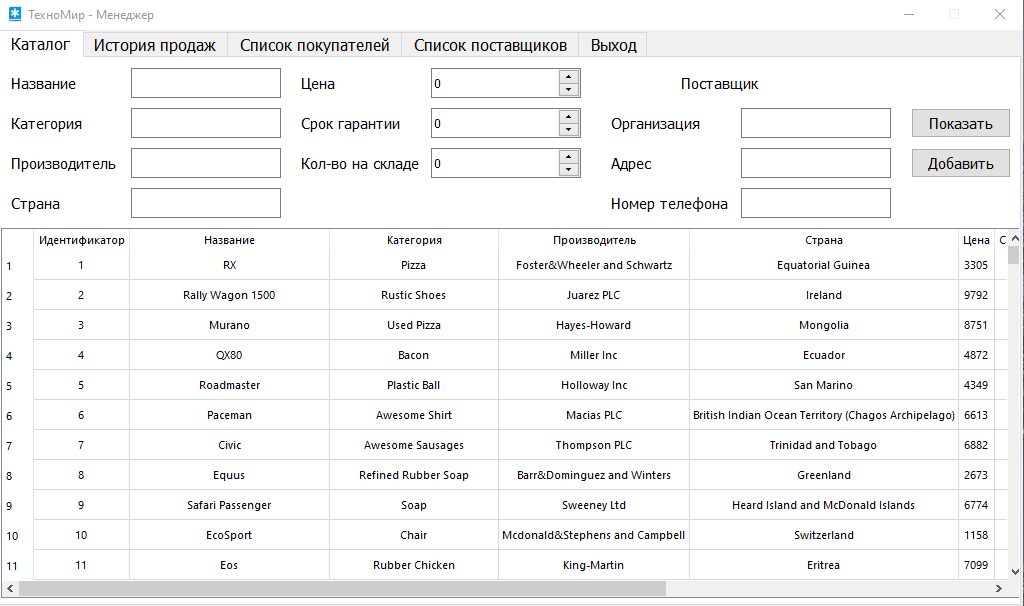
\includegraphics[width=0.95\textwidth]{img/manager_cat.png}
		\caption{Окно просмотра каталога товаров для менеджера}
		\label{tech:mancat}}
\end{figure}

Менеджер имеет возможность переключиться на вкладку просмотра истории продаж магазина. Указав минимальную сумму заказа и интересующий его временной период, менеджер может увидеть все заказы, подходящие под эти параметры. Окно просмотра истории продаж для менеджера представлено на рисунке \ref{tech:mansales}.

\begin{figure}[H]
	\centering{
		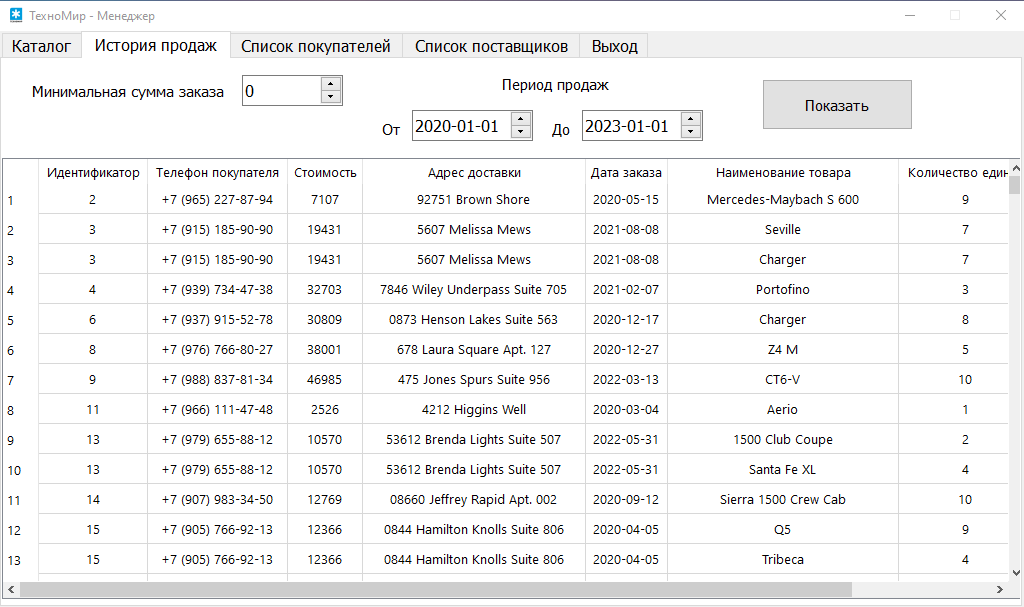
\includegraphics[width=0.95\textwidth]{img/manager_sales.png}
		\caption{Окно просмотра истории продаж}
		\label{tech:mansales}}
\end{figure}

Следующая возможность менеджера -- просмотр полного списка клиентов магазина. Доступна фильтрация по минимальной общей сумме трат в магазине. Окно просмотра списка покупателей показано на рисунке \ref{tech:manclients}.

\begin{figure}[H]
	\centering{
		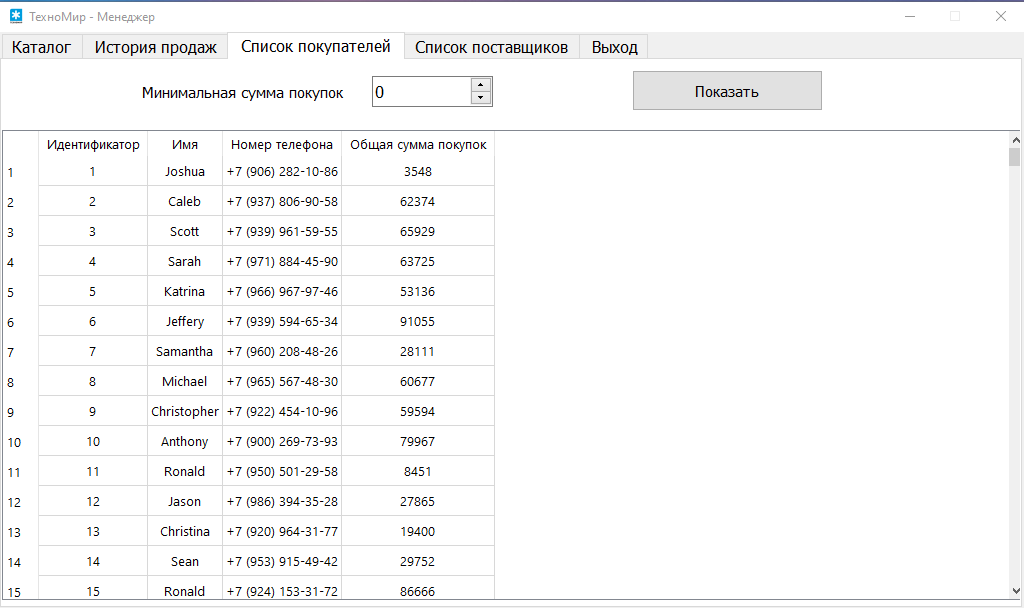
\includegraphics[width=0.95\textwidth]{img/manager_clients.png}
		\caption{Окно просмотра списка покупателей}
		\label{tech:manclients}}
\end{figure}

Последняя информативная вкладка в интерфейсе менеджера позволяет просмотреть список поставщиков товаров. Менеджер может найти сведения о нужном поставщике по названию организации. Окно просмотра списка поставщиков показано на рисунке \ref{tech:mansups}.

\begin{figure}[H]
	\centering{
		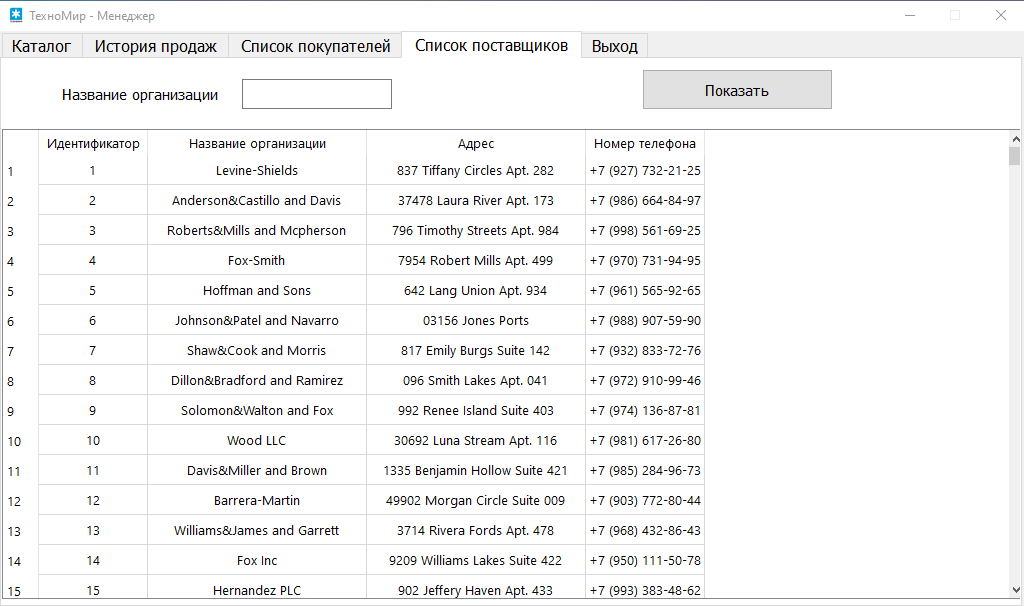
\includegraphics[width=0.95\textwidth]{img/manager_suppliers.png}
		\caption{Окно просмотра списка поставщиков}
		\label{tech:mansups}}
\end{figure}

Если войти в систему как покупатель, то открывается доступ к просмотру каталога товаров с возможностью добавления их в корзину в нужном количестве. Покупатель также может искать товары по интересующим его параметрам, для этого необходимо заполнить поля значениями для поиска. Окно просмотра каталога товаров для покупателя представлено на рисунке \ref{tech:custcat}.

\begin{figure}[H]
	\centering{
		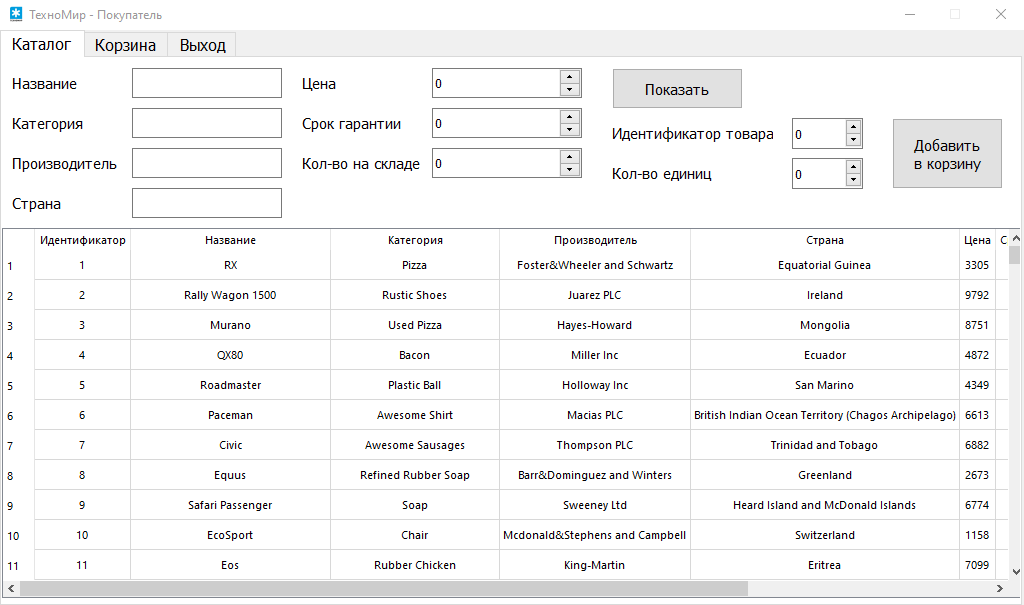
\includegraphics[width=0.95\textwidth]{img/customer_cat.png}
		\caption{Окно просмотра каталога товаров для покупателя}
		\label{tech:custcat}}
\end{figure}

После добавления нужных товаров в корзину покупатель может перейти к оформлению заказа. Для этого ему необходимо переключиться на вкладку просмотра корзины. Для осуществления заказа покупатель должен заполнить поля с контактной информацией. Также покупатель может изменить содержимое корзины, удалить ошибочно добавленные товары и внести другие. Окно просмотра корзины представлено на рисунке \ref{tech:custcart}.

\begin{figure}[H]
	\centering{
		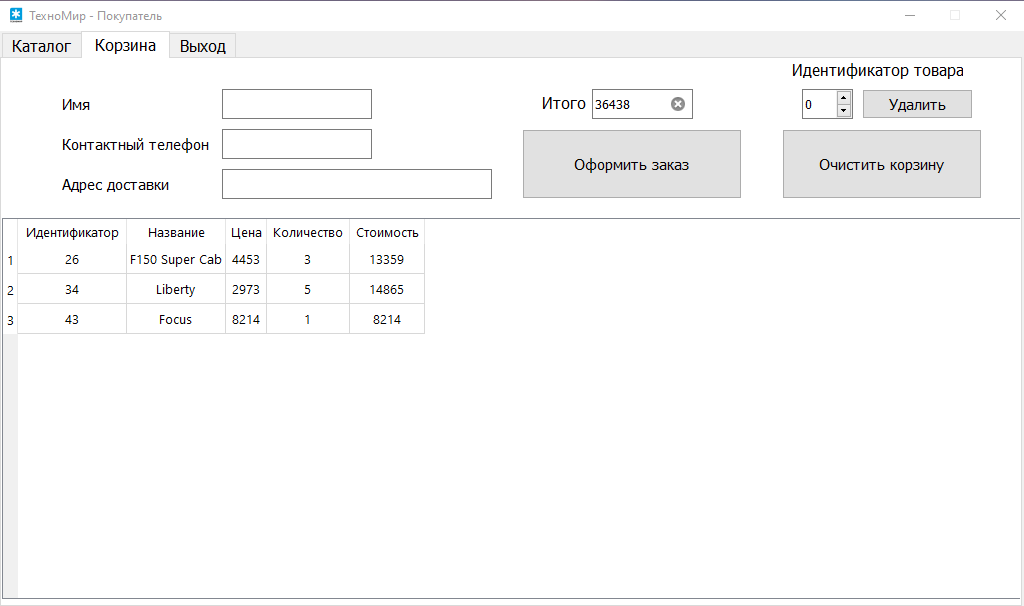
\includegraphics[width=0.95\textwidth]{img/customer_cart.png}
		\caption{Окно просмотра корзины}
		\label{tech:custcart}}
\end{figure}

\subsection*{Вывод}

В данном разделе были описаны средства реализации и структура спроектированной системы, была создана база данных магазина с ролевой моделью, а также разработано приложение с пользовательским интерфейсом.

\pagebreak